% !TEX encoding = UTF-8
\documentclass[UTF8]{ctexart}

\usepackage[utf8]{inputenc}
\usepackage{graphicx}
\usepackage{geometry}
\geometry{a4paper}
\geometry{left=2.5cm,right=2.5cm,top=2.8cm,bottom=1.3cm}

\usepackage{booktabs}
\usepackage{array}
\usepackage{paralist}
\usepackage{verbatim}
\usepackage{subfig}
\usepackage{amsmath}
\usepackage{mathtools}
\usepackage{listings}
\usepackage[table]{xcolor}
\usepackage{lastpage}
\usepackage{url}

% Using hyperref for improved ref character
\usepackage[colorlinks,linkcolor=black,anchorcolor=black,
citecolor=black,CJKbookmarks=True]{hyperref}

% For picture drawing
\usepackage[all]{xy}

% For code inserting. Set features.
\lstset{
alsolanguage=matlab,
tabsize=4,
keepspaces=true,
numbers=left,
numberstyle=\tiny,
keywordstyle=\color{blue!70} \bfseries,
commentstyle=\color{red!50!green!50!blue!50},
frame=shadowbox,
breaklines,
showspaces=false,
showstringspaces=false,
showtabs=false,
rulesepcolor=\color{red!20!green!20!blue!20},
extendedchars=false,
escapeinside=``
}

% Set the font of page header
\usepackage{fancyhdr}
\pagestyle{fancy}
\lhead{传感器特性实验报告}
\chead{}
\rhead{Page \thepage/\pageref{LastPage}}
\cfoot{}
\rfoot{}
\lfoot{}

\usepackage{sectsty}

\usepackage[nottoc]{tocbibind}
\usepackage[titles,subfigure]{tocloft}
\renewcommand{\cftsecfont}{\rmfamily\mdseries\upshape}
\renewcommand{\cftsecpagefont}{\rmfamily\mdseries\upshape}

% Set number of ref to be relevent to section number
\renewcommand{\theequation}{\arabic{section}.\arabic{equation}}
\renewcommand{\thefigure}{\arabic{section}-\arabic{figure}}
\renewcommand{\thetable}{\arabic{section}-\arabic{table}}
\makeatletter
\@addtoreset{equation}{section}
\@addtoreset{figure}{section}
\@addtoreset{table}{section}
\makeatother

% Set the font of the reference
\bibliographystyle{unsrt}

% Define user\rq{}s color
\usepackage{colortbl}
\definecolor{lightgray}{gray}{.9}
\definecolor{thickgray}{gray}{.6}

\usepackage{multirow}

% 首行缩进
\usepackage{indentfirst}

% Set section numbering
\CTEXsetup[number={}]{part}
\renewcommand{\thepart}{}
\usepackage{titlesec}
\titleformat{\part}[block]{\color{blue}\huge\bfseries\filcenter}{}{1em}{}

%\usepackage{ulem}
%\usepackage{indentfirst}
%\setlength\textwidth{300.0pt}
%

% 重定义字体命令
\newcommand{\song}{\CJKfamily{song}}    % 宋体   (Windows自带simsun.ttf)
\newcommand{\fs}{\CJKfamily{fs}}        % 仿宋体 (华天字库htfs.ttf)
\newcommand{\kai}{\CJKfamily{kai}}      % 楷体   (华天字库htkai.ttf)
\newcommand{\hei}{\CJKfamily{hei}}      % 黑体   (Windows自带simhei.ttf)
\newcommand{\li}{\CJKfamily{li}}        % 隶书   (Windows自带simli.ttf)
\newcommand{\you}{\CJKfamily{you}}      % 幼圆体 (Windows自带simyou.ttf)
%%%  以上六种字体均为标准 GBK 字体, 包括 GBK 繁体字和一些不常用字, 推荐!!!

\newcommand{\xs}{\CJKfamily{xs}}
\newcommand{\shu}{\CJKfamily{shu}}      % 舒体   (方正字库fzstk.ttf)
%  \newcommand{\yourcommand}[参数个数]{内容}   [参数个数]这个是可选的。
%  例如  \newcommand{\you}{\CJKfamily{you}}  用\you 来代替 \CJKfamily{you} ,少输入很多字哦。
%字号设置
\newcommand{\chuhao}{\fontsize{42pt}{\baselineskip}\selectfont}
\newcommand{\xiaochuhao}{\fontsize{36pt}{\baselineskip}\selectfont}
\newcommand{\yihao}{\fontsize{28pt}{\baselineskip}\selectfont}
\newcommand{\xiaoyihao}{\fontsize{24pt}{\baselineskip}\selectfont}
\newcommand{\erhao}{\fontsize{21pt}{\baselineskip}\selectfont}
\newcommand{\xiaoerhao}{\fontsize{18pt}{\baselineskip}\selectfont}
\newcommand{\sanhao}{\fontsize{15.75pt}{\baselineskip}\selectfont}
\newcommand{\sihao}{\fontsize{14pt}{\baselineskip}\selectfont}
\newcommand{\xiaosihao}{\fontsize{12pt}{\baselineskip}\selectfont}
\newcommand{\wuhao}{\fontsize{10.5pt}{\baselineskip}\selectfont}
\newcommand{\xiaowuhao}{\fontsize{9pt}{\baselineskip}\selectfont}
\newcommand{\liuhao}{\fontsize{7.875pt}{\baselineskip}\selectfont}
\newcommand{\qihao}{\fontsize{5.25pt}{\baselineskip}\selectfont}
% \baselineskip | distance from bottom of one line of a paragraph to bottom of the next line.  基本行距
%  只有使用\selectfont命令之后,\fontzize{}{}的设置才能生效
%  可以用数字表示{11pt}:单倍行距
\newcommand\smallW{
\mathchoice
	{{\scriptstyle\mathcal{W}}}% \displaystyle
	{{\scriptstyle\mathcal{W}}}% \textstyle
	{{\scriptscriptstyle\mathcal{W}}}% \scriptstyle
	{\scalebox{.7}{$\scriptscriptstyle\mathcal{W}$}}%\scriptscriptstyle
}


\begin{document}
%%%%%%%%%%%%%%%%%%%%%%%%%%%%封面与目录%%%%%%%%%%%%%%%%%%%%%%%%%%%%%%
\begin{titlepage}
\begin{center}
% Upper part of the page

\includegraphics[width=0.25\textwidth]{resource/logo.jpg}\\[1cm]
\textsc{\LARGE Department of Automation}\\[1.5cm]
\fs{\Large 人工智能导论第二次大作业}\\[0.5cm]
% Title
\hrulefill
\\[0.8cm]{\centering \huge \hei 基于特征选择和深度神经网络的杯子自动分类}\\[0.4cm]
\hrulefill
\\[4cm]

% Author and supervisor
\begin{tabbing}       %tabbing  列表

 \hspace*{5cm} \= \hspace{2.6cm} \= \kill
 % \=     in tabbing environment, sets a tab stop
 % \kill  in a\tabbing environment, deletes previous line so tabs can be set without outputting text.
 % \>     in tabbing environment is a forward tab.

\>{\fs\sihao\textbf {班\hspace{1cm}级 \ \ :}}\>  {\centering\fs\sihao\textbf{~~~~~~~~~自~~3~2}} \\
\\
\>{\fs\sihao\textbf {姓\hspace{1cm}名 \ \ :}}\>  {\centering\fs\sihao\textbf{~陈~昊~楠~(2013011449)}}\\
\\
\>{\fs\sihao\textbf {同~~组~~人 \ \ :}}\>  {\centering\fs\sihao\textbf{~赵~~~~~~灿~(2013011439)}}\\
\\
\>{\fs\sihao\textbf {授课教师 \ \ :}}\>  {\centering\fs\sihao\textbf{~~~~~~~~张~长~水}} \\

\end{tabbing}
\vfill
{\large \today}
\end{center}
\end{titlepage}

\tableofcontents
\clearpage

%%%%%%%%%%%%%%%%%%%%%%%%%%正文部分%%%%%%%%%%%%%%%%%%%%%%%%%%%%%%%%%%

\section{实验说明}
\subsection{程序语言与依赖库}
	实验程序使用Python编写,依赖以下库函数:
	\begin{enumerate}
	\item Scikit-learn \url{http://scikit-learn.org/},用于提供特征分类的机器学习方法;
	\item Pandas \url{http://pandas.pydata.org/},用于数据结果生成;
	\item TensorFlow \url{https://www.tensorflow.org/},用于深度学习模型搭建;
	\item OpenCV \url{http://opencv.org/},用于读取和预处理图片。
	\end{enumerate}
	关于如何安装以上依赖库,参见 \url{https://github.com/chaonan99/university_homework/tree/AI_cup_class}。

\subsection{程序运行环境}
	运行环境如表\ref{tab:environment}。

	\begin{table}[htbp]
	\centering
	\begin{tabular}{cc}
	\hline
	\multirow{2}*{System}&  {\ttfamily Ununtu 14.04} \\
	 & {\ttfamily Ununtu 16.04} \\
	Python & 2.7 / 3.5\\
	TensorFlow  &  $0.10.0$ \\
	Cuda & v8.0 \\
	cudnn & v5.0.5 \\
	\hline
	\end{tabular}
	\caption{程序运行环境}
	\label{tab:environment}
	\end{table}

\subsection{需求分析}
	本次作业要求利用{\ttfamily SVM}、神经网络或其他方法实现对杯子数据的分类功能。其中所有数据均为$3*128*128$大小的实拍杯子图片。杯子按不同特征分为$6$类,如表\ref{tab:cupclass}

	\begin{table}[htbp]
	\centering
	\begin{tabular}{ccc}
	\toprule
	类别 & 特征 & 材质 \\
	\midrule
	1 & 有盖无把 & 塑料 \\
	2 & 有盖 & 金属 \\
	3 & 无盖有把 & \multicolumn{1}{p{2.6cm}}{塑料、纸、玻璃、陶瓷、金属} \\
	4 & 无盖无把 & 硬塑料 \\
	5 & 形状不规则 & 软塑料 \\
	6 & 固体容器 & 硬塑料 \\
	\bottomrule
	\end{tabular}
	\caption{杯子类别情况}
	\label{tab:cupclass}
	\end{table}

	其中,训练集数据2858个,测试集数据904个。因此本次作业主要分为四个步骤:搭建分类模型;使用训练集训练分类模型;使用分类模型对测试集进行分类;对比分析分类结果与准确率。

\subsection{组员分工}
组员的分工如表\ref{tab:job}。

\begin{table}[htbp]
\centering
\begin{tabular}{cc}
\hline
实现算法 & 负责人 \\
\hline
MLP & 陈昊楠 \\
Bayes & 陈昊楠 \\
LDA & 陈昊楠 \\
dCNN & 陈昊楠、赵灿 \\
PCA & 赵灿 \\
SVM & 赵灿 \\
特征选择方法 & 陈昊楠 \\
报告撰写 & 陈昊楠、赵灿 \\
\hline
\end{tabular}
\caption{组员分工}
\label{tab:job}
\end{table}

\subsection{测试接口说明}
使用预提取的特征,Python2 运行
\begin{lstlisting}
python cup_prefeat.py --test_pickle /path/to/test/pickle
\end{lstlisting}
Python3 运行
\begin{lstlisting}
python3 cup_prefeat_3.py --test_pickle /path/to/test/pickle
\end{lstlisting}
经过一段时间,将输出测试准确率。
使用深度神经网络的代码在{\ttfamily cup\_net\_example}下,参见 \url{https://github.com/chaonan99/university_homework/tree/AI_cup_class}。

\section{实验方法}
本实验采用了两种途径进行杯子分类,从预先提取的特征中,采用各种分类器进行分类,和直接从原图训练卷积神经网络进行分类。

\subsection{基于预提取特征}
实验中给出了256维的杯子特征。对于这些特征,我们使用了多种分类器,包括最小错误率贝叶斯分类器,{\ttfamily Fisher}线性判别,支持向量机,人工神经网络,决策树等方法。实验中还对256维特征进行了基于统计量、基于准则函数和基于交叉检验的特征选择方法并在分类器上测试结果。{\ttfamily PCA}作为一种有效的降维手段也在实验中进行了尝试。

\subsection{Fisher线性分类器}
	多类的线性判别方法是基于二分类的。二分类的线性判别函数的一般表达式为
	\begin{equation}
	f(\mathbf{x}) = \mathbf{w}^\top \mathbf{x} + b
	\label{eq:LDA}
	\end{equation}
	其中 $\mathbf{w}$ 和 $b$ 是由训练样本确定的参数。对于一个测试样本 $\mathbf{x^{(i)}}$,计算其 $f(\mathbf{x^{(i)}})$ 值,依据其与 $0$ 的大小就可以判定类别。上式中 $b$ 仅用于调整阈值,而投影向量 $\mathbf{x^{(i)}}$ 是决定分类器效果的关键。

	Fisher线性判别的思想是,选择投影方向,使得投影后两类相隔尽可能远,而同时每一类内部的样本又尽可能聚集。其数学表达为
	\begin{equation}
	\max J_F(w)=\frac{\tilde{S}_b}{\tilde{S}_w}=\frac{(\tilde{m}_1-\tilde{m}_2)^2}{\tilde{S}_1^2+\tilde{S}_2^2}
	\end{equation}
	其中 $\tilde{m}_1, \tilde{m}_2$ 为两类投影后的均值
	\begin{equation}
	\tilde{m}_i=\frac1{N_i}\sum_{y_j\in \mathcal{Y}_i}y_j=\frac1{N_i}\sum_{x_j\in \mathcal{X}_i}w^\top\boldsymbol{x_j}=w^\top\boldsymbol{\mu}_i\quad i=1,2
	\end{equation}
	$\tilde{S}_1, \tilde{S}_2$为两类投影后的的类内离散度
	\begin{equation}
	\tilde{S}_i^2=\sum_{y_j\in \mathcal{Y}_i}(y_j-\tilde{m}_i)^2\quad i=1,2
	\end{equation}
	可以证明,在该准则下,投影方向 $\mathbf{w}$ 为
	\begin{equation}
	\mathbf{w} = \alpha \cdot (\mathbf{S}_1 + \mathbf{S}_2)^{-1} (\boldsymbol{\mu}_1 - \boldsymbol{\mu}_2)
	\end{equation}
	阈值为
	\begin{equation}
	b = -\frac12(\boldsymbol{\mu}_1 + \boldsymbol{\mu}_2)(\mathbf{S}_1 + \mathbf{S}_2)^{-1} (\boldsymbol{\mu}_1 - \boldsymbol{\mu}_2)-\ln\frac{P(\omega_1)}{P(\omega_2)}
	\end{equation}
	其中 $\mathbf{S}_1, \mathbf{S}_2$ 为类内离散度矩阵
	\begin{equation}
	\mathbf{S}_i=\sum_{x_j\in \mathcal{X}_i}(\boldsymbol{x_j}-\boldsymbol{\mu}_i)(\boldsymbol{x_j}-\boldsymbol{\mu}_i)^\top
	\end{equation}

	将二分类器运用于多类问题,有两种设计思路。假设类别数为$K$,
	\begin{enumerate}
	\item 设计 $K-1$ 个二分类器,每个分类器将某一类和其他类分开。如果如果样本没有分到 $K-1$ 个类中,则属于第 $K$ 类。这样设计的分类器可能产生歧义,即一个样本可能被分到多类中。
	\item 为多类中的每两对逐对分类。一共 $\frac{K(K-1)}{2}$ 个分类器。
	\end{enumerate}

	以上假设二分类的线性判别器只能输出类别信息。而多数基于线性判别函数的分类器的判别函数值可以作为距离分类器面的远近。因此可以有第三种设计方法,即由训练数据产生 $K$ 个判别函数(式 \ref{eq:LDA}),分类时比较判别函数值,取最大者作为类别结果。

\subsubsection{Bayes最小错误率分类}
	该方法假设每一类下的所有特征服从多维正态分布,每类的判别函数采用条件概率的负对数形式。设第 $i$ 类下正态分布的均值、协方差为 $\mu_i,\Sigma_i\quad$,则判别函数为
	\begin{equation}
	\label{eq:discrim}
		\begin{split}
		g_i(\mathbf{x})&=-\frac{1}{2}(\mathbf{x}-\mu_i)^\mathbf{T}\Sigma^{-1}_i(\mathbf{x}-\mu_i)-\frac{d}{2}\ln 2\pi-\frac{1}{2}\ln|\Sigma_i|+\ln P(\omega_i) \\
		{}&=\mathbf{x^TW}_i\mathbf{x}+\mathbf{w^T}_i\mathbf{x}+\smallW_{i0}
		\end{split}
	\end{equation}
	其中,
	\begin{align}
		\mathbf{W}_i&=-\frac12\Sigma_i^{-1}\\
		\mathbf{w}_i&=\Sigma_i^{-1}\mu_i\\
		\smallW_{i0}&=-\frac12\mu_i^\mathbf{T}\Sigma_i^{-1}\mu_i-\frac12\ln|\Sigma_i|+\ln P(\omega_i)
	\end{align}

	第 $i,j$ 两类的决策边界为 $g_i(\mathbf{x})=g_j(\mathbf{x})$,即
	\begin{equation}
	\label{eq:bayes}
	-\frac12[(x-\mu_i)^\top\Sigma_i^{-1}(x-\mu_i)-(x-\mu_j)^\top\Sigma_j^{-1}(x-\mu_j)]-\frac12\ln \frac{|\Sigma_i|}{|\Sigma_j|}+\ln\frac{P(\omega_i)}{P(\omega_j)}=0
	\end{equation}

\subsubsection{SVM}
支持向量机(support vector machine,简称SVM)是一种二分类模型,其基本模型定义为特征空间上间隔最大的线性分类器,其学习策略便是间隔最大化,最终可转化为一个凸二次规划问题的求解。
以二维空间为例,线性可分样本分布如图\ref{fig:SVM}所示。线性判别函数为$g(x)=wx+b$,对$g(x)$进行归一化,使得两类样本中距离最优平面最近的样本满足$|g(x)|=1$,由此可以得到两类样本的间隔为$2/|| w ||$。

\begin{figure}[htbp]
\centering
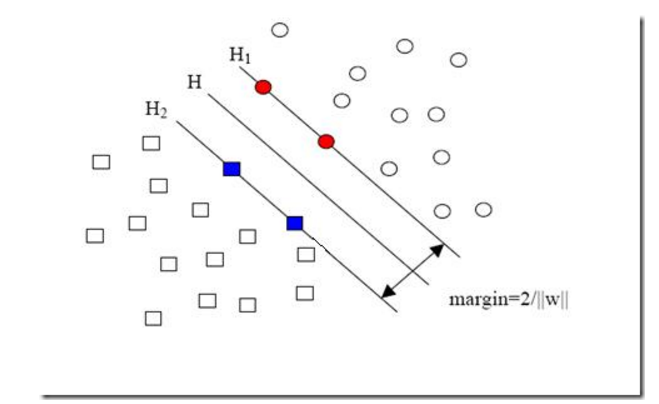
\includegraphics[width=6cm]{resource/SVM.png}
\caption{两类样本线性可分情况SVM模型}
\label{fig:SVM}
\end{figure}

为了最大化两类样本的间隔,需要最小化|| w ||,为了正确划分样本,需要满足:
\begin{equation}w\cdot {{x}_{i}}+b\ge 1,\text{ }if\text{ }{{y}_{i}}=1\end{equation}
\begin{equation}w\cdot {{x}_{i}}+b\le \text{-}1,\text{ }if\text{ }{{y}_{i}}=\text{-}1\end{equation}
由此可以转换为如下优化方程:
\begin{align}
\min \quad& \frac{1}{2}||w|{{|}^{2}}\\
s.t.\quad & {{y}_{i}}(w\cdot {{x}_{i}}+b)\ge 1,i=1,2...N
\end{align}

上述问题可以利用拉格朗日乘子转换为如下对偶问题:
\begin{align}
\max \quad & W(a\text{)=}\sum\limits_{i=1}^{N}{{{a}_{i}}}-\frac{1}{2}\sum\limits_{i,j}{{{a}_{i}}}{{a}_{j}}{{y}_{i}}{{y}_{j}}{{x}_{i}}\cdot {{x}_{j}} \\
s.t.\quad & \sum\limits_{i=1}^{N}{{{a}_{i}}}{{y}_{i}}=0 \\
& {{a}_{i}}\ge 0,i=1,2,...N
\end{align}

得到优化问题的最优解后,可以根据决策函数$sign(h(x))$判断测试样本的类别。$sign(.)$为符号函数,$x_l,\quad l=1,2,…,m$ 为支持向量(满足 $\alpha_l>0$), $b$可以使用任意支持向量带入下式求解得到:
\begin{equation}
h(x)=\sum\limits_{l=1}^{m}{{{a}_{l}}}{{y}_{l}}x\cdot {{x}_{l}}+b
\end{equation}

与LDA方法类似,SVM也可以由二分类推广到多分类。

\subsubsection{MLP神经网络}
	如图\ref{fig:sn},对于单个神经元有
	\begin{equation}
	h_{W,b}(x)=f(W^\top x+b)
	\end{equation}
	其中,$f(\cdot)$ 为激活函数,可以取为 {\ttfamily Sigmoid,tanh,Relu} 等形式
	\begin{figure}[htbp]
	\centering
	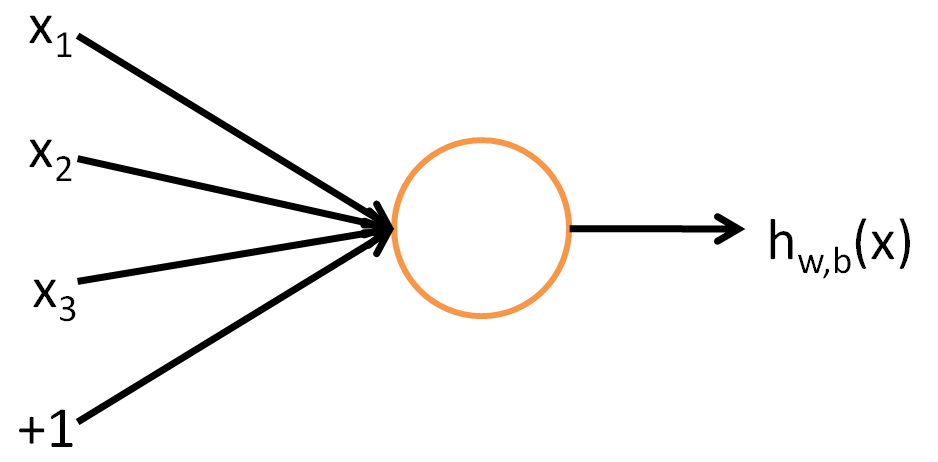
\includegraphics[width=8cm]{resource/SingleNeuron.png}
	\caption{网络神经元}
	\caption*{\small 来源: \url{http://ufldl.stanford.edu/tutorial/supervised/MultiLayerNeuralNetworks/}}
	\label{fig:sn}
	\end{figure}

	\begin{figure}[htbp]
	\centering
	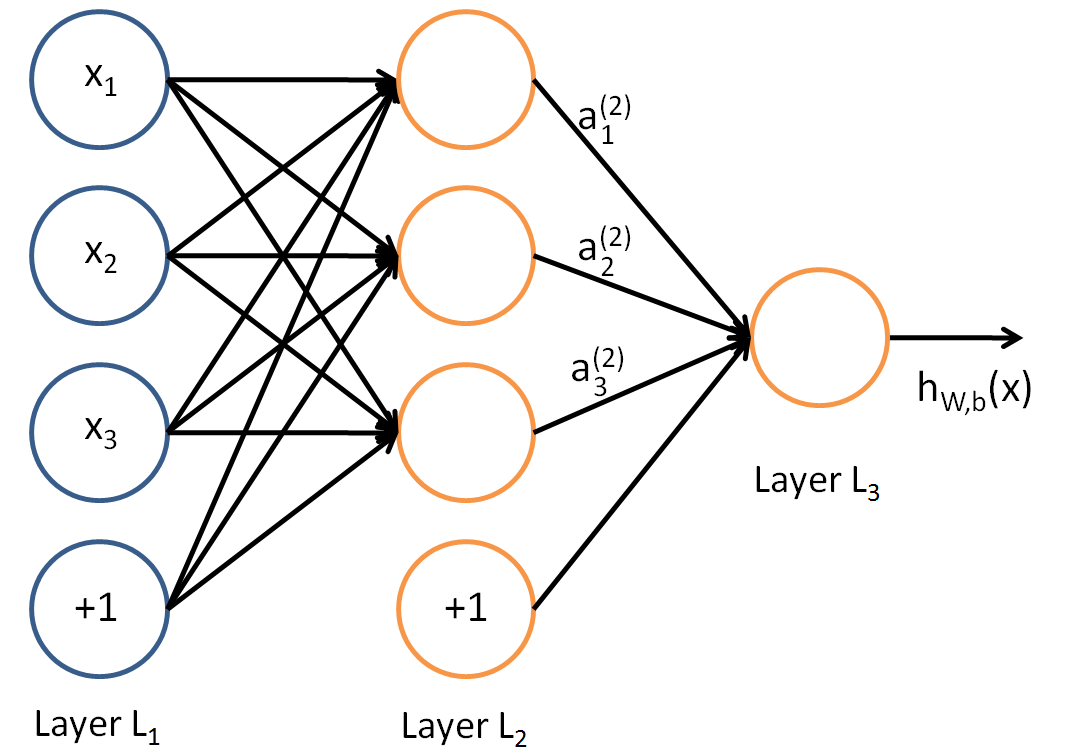
\includegraphics[width=8cm]{resource/Network331.png}
	\caption{单层神经网络}
	\caption*{\small 来源: \url{http://ufldl.stanford.edu/tutorial/supervised/MultiLayerNeuralNetworks/}}
	\label{fig:n331}
	\end{figure}

	将多个神经元连接为神经网络模型,如图\ref{fig:n331},网络前向传播公式为:
	\begin{align}
	a_1^{(2)} &= f(W_{11}^{(1)}x_1 + W_{12}^{(1)} x_2 + W_{13}^{(1)} x_3 + b_1^{(1)})  \\
	a_2^{(2)} &= f(W_{21}^{(1)}x_1 + W_{22}^{(1)} x_2 + W_{23}^{(1)} x_3 + b_2^{(1)})  \\
	a_3^{(2)} &= f(W_{31}^{(1)}x_1 + W_{32}^{(1)} x_2 + W_{33}^{(1)} x_3 + b_3^{(1)})  \\
	h_{W,b}(x) &= a_1^{(3)} =  f(W_{11}^{(2)}a_1^{(2)} + W_{12}^{(2)} a_2^{(2)} + W_{13}^{(2)} a_3^{(2)} + b_1^{(2)})
	\end{align}

	写成矩阵形式:
	\begin{align}
	z^{(l+1)} &= W^{(l)} a^{(l)} + b^{(l)}   \\
	a^{(l+1)} &= f(z^{(l+1)})
	\end{align}

	多个这样的层即可连接成多层神经网络,如图\ref{fig:n3322}。网络输出层与期望输出之间可以建立损失函数,并使用梯度下降法使输出逼近期望的输出。常用的$L_2$损失函数为
	\begin{align}
	J(W,b; x,y) = \frac{1}{2} \left\| h_{W,b}(x) - y \right\|^2.
	\end{align}

	\begin{figure}[htbp]
	\centering
	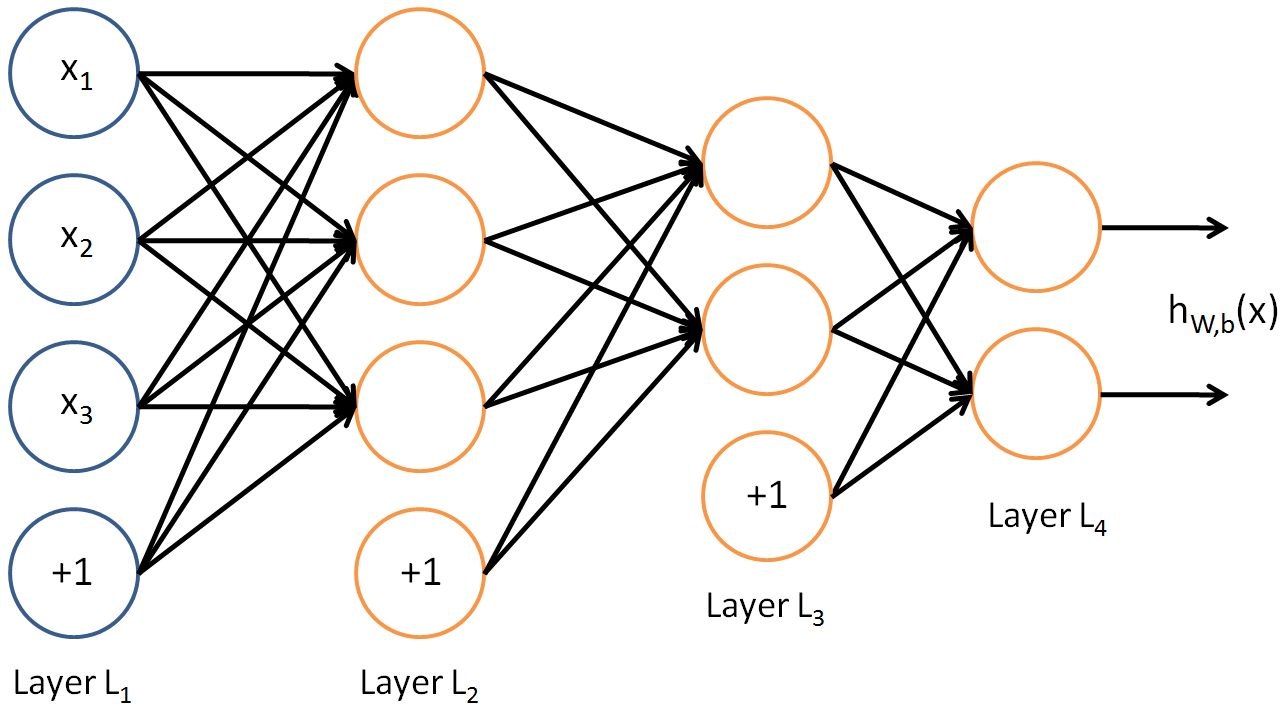
\includegraphics[width=8cm]{resource/Network3322.png}
	\caption{多层神经网络}
	\caption*{\small 来源: \url{http://ufldl.stanford.edu/tutorial/supervised/MultiLayerNeuralNetworks/}}
	\label{fig:n3322}
	\end{figure}

	使用多层神经网络进行分类时,输出层具有和类别数相同的神经元个数,并且接一个{\ttfamily Softmax}分类器,即
	\begin{equation}
	P(y = k | x ; \theta) = \frac{\exp(\theta^{(k)\top} x)}{\sum_{j=1}^K \exp(\theta^{(j)\top} x) },
	\end{equation}
	其中,$y \in \{1,\ldots,K\}$,$K$为类别数目,$x$在这里表示最后一级隐藏层的输出,准备进入输出层。{\ttfamily Softmax}分类器将一组输出转化为维数相同的概率分布,因此可以作为各类的概率表示。{\ttfamily Softmax}分类器常常结合{\ttfamily Cross Entropy}损失函数,
	\begin{align}
	J(\theta) &= - \left[ \sum_{i=1}^m   (1-y^{(i)}) \log (1-h_\theta(x^{(i)})) + y^{(i)} \log h_\theta(x^{(i)}) \right] \\
	&= - \left[ \sum_{i=1}^{m} \sum_{k=0}^{1} 1_k\left(y^{(i)}\right) \log P(y^{(i)} = k | x^{(i)} ; \theta) \right]
	\end{align}

	这里$i$为样本标号,$x^{(i)}$代表第$i$个样本,$y^{(i)}$为第$i$个样本的真实类别,,$h_\theta(\cdot)$代表神经网络模型的运算,它将$x^{(i)}$映射为一组概率分布,$1_k\left(y^{(i)}\right)$为{\ttfamily indicator}函数,定义为
	\begin{equation}\mathbf{1}_A(x) :=
	\begin{cases}
	1 &\text{if } x \in A, \\
	0 &\text{if } x \notin A.
	\end{cases}
	\end{equation}

\subsubsection{特征选择方法}
	一般的特征选择问题的解决思路是,构造一个准则函数,对一组特征打分,并搜索使得准则最优的特征组合。这种方式搜索空间很大,实际问题中可以采用如下几个思路:
	\begin{enumerate}
	\item 对每个特征,单独计算一个特征与目标分类的函数$f(X_i, y)$,该函数的值被称为p值。根据这个值对特征进行排序,并选择最优的几个特征。
	\item 从一个特征集合中尝试删去部分特征,构造树状结构,并使用分支定界法进行搜索。
	\item 与分类器集成在一起,而不是采用单独的可分性准则。例如{\ttfamily SVM-RFE}方法。
	\end{enumerate}

\subsubsection{PCA原理}
主成分分析是数学上对数据降维的一种方法。其基本思想是设法将原来众多的具有一定相关性的$p$个特征$X_1, X_2, \dots,X_P$,使用特征提取的方法重新合成一组较少个数的互不相关的新特征$Y_1, Y_2,\dots,Y_m$。新特征应能最大程度的反映原特征$X_p$所包含的信息,同时保证新特征之间保持相互无关(信息不重叠)。
设F1表示原始特征的第一个线性组合所形成的主成分指标,即${{Y}_{1}}={{a}_{11}}{{X}_{1}}+{{a}_{21}}{{X}_{2}}+...+{{a}_{p1}}{{X}_{p}}$。而每一个主成分所提取的信息量可用其方差来度量,其方差$Var(Y_1)$越大表示$Y_1$包含的信息越多。因此第一主成分$Y_1$所含的信息量应最大,即是$X_1, X_2, \dots,X_P$的所有线性组合中方差最大的;选取第二个主成分指标$Y_2$时,为有效地反映原信息,应避免Y1已有的信息出现在$Y_2$中,即其协方差$\operatorname{cov}({{Y}_{1}},{{Y}_{2}})=0$;依此类推构造出的$Y_1, Y_2,\dots,Y_m$,依次原变量的第一、第二、…、第$m$个主成分。
\begin{equation}\left\{ \begin{matrix}
   {{F}_{1}}={{a}_{11}}{{X}_{1}}+{{a}_{12}}{{X}_{2}}+...+{{a}_{1p}}{{X}_{p}}  \\
   {{F}_{2}}={{a}_{21}}{{X}_{1}}+{{a}_{22}}{{X}_{2}}+...+{{a}_{2p}}{{X}_{p}}  \\
   ......  \\
   {{F}_{m}}={{a}_{m1}}{{X}_{1}}+{{a}_{m2}}{{X}_{2}}+...+{{a}_{mp}}{{X}_{p}}  \\
\end{matrix} \right.
\end{equation}
主成分分析的具体步骤如下:
\begin{enumerate}
\item 计算样品数据的协方差矩阵
\begin{equation}
\Sigma ={{[{{s}_{ij}}]}_{p\times p}}
\end{equation}
其中,
\begin{equation}
{{s}_{ij}}=\frac{1}{n-1}\sum\limits_{k=1}^{n}{({{x}_{ki}}-{{{\bar{x}}}_{i}})({{x}_{kj}}-{{{\bar{x}}}_{j}})} \quad i,j=1,2,\ldots p
\end{equation}
\item 求出$\Sigma$的特征值${{\lambda }_{i}}$及相应的正交化单位特征向量${{a}_{i}}$,$\Sigma$的前$m$个较大的特征值$\lambda_1\geq \lambda_2\geq \dots\geq \lambda_m>0$,就是前m个主成分对应的方差,${{\lambda }_{i}}$对应的单位特征向量${{a}_{i}}$就是主成分Fi的关于原变量的系数,则原变量的第$i$个主成分$F_i$为:
\begin{equation}
F_i ={{a}_{i}}'X
\end{equation}
\item 选择主成分
    最终要选择几个主成分,即$F_1, F_2,\dots,F_m$中$m$的确定是通过方差(信息)累计贡献率$G(m)$来确定
\begin{equation}
G(m)=\sum\limits_{i=1}^{m}{{{\lambda }_{i}}}/\sum\limits_{k=1}^{p}{{{\lambda }_{k}}}
\end{equation}
当累积贡献率大于设定阈值时,认为此时已经足够反映原始信息,此时m就是抽取的前m个主成分。
\end{enumerate}

\subsection{由原始图片学习特征}
实验中使用了{\ttfamily TensorFlow}进行模型的搭建和训练。{\ttfamily TensorFlow}是谷歌基于{\ttfamily DistBelief}进行研发的第二代人工智能学习系统,其命名来源于本身的运行原理。{\ttfamily TensorFlow} 是一个编程系统, 使用图来表示计算任务。 图中的节点被称之为 op (operation 的缩写), 一个 op 获得 0 个或多个 {\ttfamily Tensor}, 执行计算, 产生 0 个或多个 {\ttfamily Tensor}。每个 {\ttfamily Tensor} 是一个类型化的多维数组,{\ttfamily Flow}(流)意味着基于数据流图的计算,{\ttfamily TensorFlow}为张量从图象的一端流动到另一端计算过程,是将复杂的数据结构传输至人工智能神经网中进行分析和处理过程的系统。
\subsubsection{卷积神经网络原理}
	卷积神经网络(Convolutional Neural Networks)是一个多层的神经网络,每层由多个二维平面组成,而每个平面由多个独立神经元组成。卷积神经网络的结构如图\ref{fig:CNN}所示:

	\begin{figure}[htbp]
	\centering
	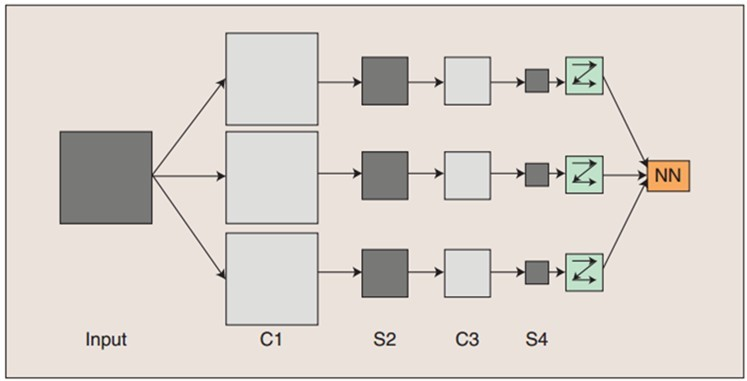
\includegraphics[width=8cm]{resource/CNN_structure.jpg}
	\caption{卷积神经网络的结构图}
	\label{fig:CNN}
	\end{figure}

	输入图像通过多个可训练的滤波器和可加偏置进行卷积,卷积后在C1层产生相应特征映射图,再加权值($W$)和偏置($b$),通过激活函数({\ttfamily Sigmoid, Relu}等)得到S2层的特征映射图。这些映射图再经过滤波输入到下一层级。最终,像素值被光栅化,并连接成一个向量输入到传统的神经网络,最后经过{\ttfamily Softmax}分类器得到输出。

	由于CNNs的结构特性,每一个映射面上的神经元共享权值,因而减少了网络自由参数的个数,降低了网络参数选择的复杂度。卷积神经网络中的每一个特征提取层(C层)都紧跟着一个用来求局部平均与二次提取的池化层(pooling,图中的S层),这种特征提取结构使网络在识别时对输入样本有较高的畸变容忍能力。
	其中,滤波过程示意如图\ref{fig:CNN_f}:

	\begin{figure}[htbp]
	\centering
	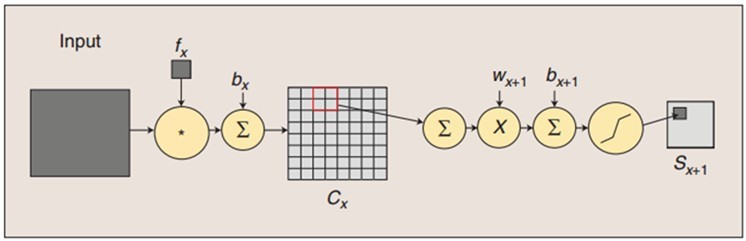
\includegraphics[width=10cm]{resource/CNN_filter.jpg}
	\caption{卷积神经网络的滤波过程}
	\label{fig:CNN_f}
	\end{figure}

	CNNs的训练算法主要包括4步,两个阶段
	第一阶段,前向传播阶段:
	\begin{enumerate}
	\item 从样本集中取一个样本$(X,Y_p)$,将X输入网络;
	\item 计算相应的实际输出Op。
	\end{enumerate}

	在此阶段,信息从输入层经过逐级的变换,传送到输出层。这个过程也是网络在完成训练后正常运行时执行的过程。在此过程中,网络执行的是计算(实际上就是输入与每层的权值矩阵相点乘,得到最后的输出结果):
	\begin{equation}
	Op=F_n(\dots(F_2(F_1(X_pW_1)W_2)\dots)W_n)
	\end{equation}

	第二阶段,反向传播阶段
	\begin{enumerate}
	\item 算实际输出Op与相应的理想输出$Y_p$的差;
	\item 按极小化误差的方法反向传播调整权矩阵$W$和偏置$b$,采用梯度下降的方法逼近目标网络结构。
	\end{enumerate}

	卷积神经网络相较于一般BP结构神经网络,由于权重共享,可以减少网络的训练参数,使神经网络结构变得更简单适应性更强。

\subsubsection{网络结构}
实验中采用了两种卷积神经网络模型。一种是类似于LeNet-5的结构,一种是AlexNet。实验中使用的简单神经网络结构如图\ref{fig:Lenet}。AlexNet的各层细节如表\ref{tab:AlexNet}。

\begin{figure}[htbp]
\centering
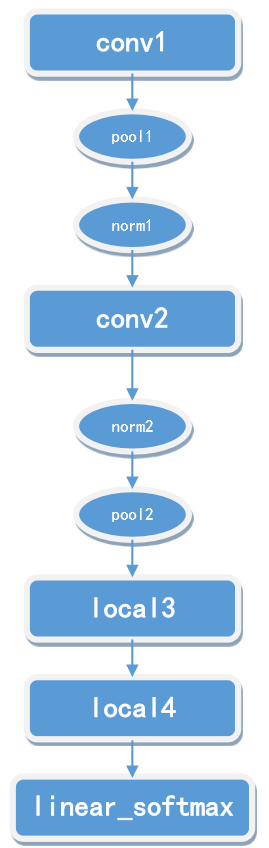
\includegraphics[width=3cm]{resource/Lenet.png}
\caption{简单卷积神经网络结构}
\label{fig:Lenet}
\end{figure}

\begin{table}[htbp]
\centering
\begin{tabular}{ccccccccc}
\hline
Layer & \textbf{1} & \textbf{2} & \textbf{3} & \textbf{4} & \textbf{5} & \textbf{6} & \textbf{7} & \textbf{8} \\
\hline
Type & c+m+n & c+m+n & c & c & c+m & full & full & full \\
Channels & 96 & 256 & 384 & 384 & 256 & 4096 & 4096 & 1000 \\
Filter Size & 11*11 & 5*5 & 3*3 & 3*3 & 3*3 & - & - & - \\
Conv Stride & 4*4 & 1*1 & 1*1 & 1*1 & 1*1 & - & - & - \\
Pooling Size & 3*3 & 3*3 & - & - & 3*3 & - & - & - \\
Pooling Stride & 2*2 & 2*2 & - & - & 2*2 & - & - & - \\
Padding Size & 2*2 & 1*1 & 1*1 & 1*1 & 1*1 & - & - & - \\
\hline
\end{tabular}
\caption{AlexNet网络结构,其中Type中 convolution,m表示 max pooling,n表示 LRN norm}
\label{tab:AlexNet}
\end{table}

\section{实验结果}
\subsection{预提取特征分类}

\begin{table}[htbp]
\centering
\begin{tabular}{ccccccc}
\toprule
Methods &   Bayes &     LDA &    LSVM & RBF SVM &     MLP &   DTree \\
\midrule
train &  73.85\% &  89.67\% &  94.96\% &  99.79\% &  99.79\% &  99.82\% \\
test &  58.78\% &  74.48\% &  76.46\% &  76.24\% &  81.55\% &  54.25\% \\
\bottomrule
\end{tabular}
\caption{不同分类方法在训练、测试集上的准确率}
\label{tab:classify}
\end{table}

由以上数据可见,多层感知器(MLP)的分类效果比较好,线性判别LDA、线性SVM和RBF核SVM也能取得可比的效果,但使用Bayes分类器和决策树的分类方法效果不佳。

\subsection{统计量选择特征}
使用$\chi^2$检验、$F$检验和互信息量来检验特征与分类目标的相关性,由此选取100个特征进行分类,训练集的准确率如表\ref{tab:sel_train},测试集的准确率如表\ref{tab:sel_test}。表中第一行为未进行特征选择的情况。由表可见,选取部分特征进行分类使分类准确率有所下降。

\begin{table}[htbp]
\centering
\begin{tabular}{ccccccc}
\toprule
{} &   Bayes &     LDA &    LSVM & RBF SVM &     MLP &   DTree \\
\midrule
no selection &  73.85\% &  89.67\% &  94.96\% &  99.79\% &  99.79\% &  99.82\% \\
$\chi^2$ test &  68.78\% &  78.75\% &  82.60\% &  96.22\% &  99.79\% &  99.82\% \\
$F$ test &  69.34\% &  78.61\% &  82.74\% &  96.29\% &  99.79\% &  99.82\% \\
Mutual Info &  68.08\% &  76.86\% &  81.13\% &  96.95\% &  99.79\% &  99.82\% \\
\bottomrule
\end{tabular}
\caption{基于p值的特征选择方法训练集准确率}
\label{tab:sel_train}
\end{table}

\begin{table}[htbp]
\centering
\begin{tabular}{ccccccc}
\toprule
{} &   Bayes &     LDA &    LSVM & RBF SVM &     MLP &   DTree \\
\midrule
no selection &  58.78\% &  74.48\% &  76.46\% &  76.24\% &  81.55\% &  53.92\% \\
$\chi^2$ test & 52.60\% &  64.42\% &  68.07\% &  67.40\% &  72.15\% &  53.92\% \\
$F$ test &      55.47\% &  64.20\% &  67.40\% &  69.39\% &  70.39\% &  56.13\% \\
Mutual Info &   52.82\% &  62.65\% &  68.62\% &  66.85\% &  74.70\% &  52.82\% \\
\bottomrule
\end{tabular}
\caption{基于p值的特征选择方法测试集准确率}
\label{tab:sel_test}
\end{table}

\subsection{PCA降维}
PCA降维后,在训练集、测试集上的准确率如表\ref{tab:PCA}。测试集上的准确率与使用所有特征相比都有所下降。

\begin{table}[htbp]
\centering
\begin{tabular}{ccccccc}
\toprule
{} &   Bayes &     LDA &    LSVM & RBF SVM &     MLP &   DTree \\
\midrule
train &  64.37\% &  87.68\% &  92.33\% &  99.79\% &  99.79\% &  99.82\% \\
test  &  48.40\% &  72.93\% &  76.24\% &  72.93\% &  76.35\% &  41.10\% \\
\bottomrule
\end{tabular}
\caption{PCA降至200维在训练、测试集上的准确率}
\label{tab:PCA}
\end{table}

\subsection{CNN深度网络}
\subsubsection{训练设置}
实验训练过程中对图片进行了数据增强处理,图片被随机截取部分区域,亮度和对比度随机进行变化。对于简单网络,输入图片大小为$24\times 24$,初始学习率为$10^{-3}$。对于AlexNet,输入图片大小为$128\times 128$,初始学习率为$10^{-4}$,每$350$个epoch学习率下降一半。对于两种方法,实验中均使用100张训练图片用作交叉验证,使用$900$张图片做测试。最终在测试集上的准确率如表\ref{tab:CNN}。

\begin{table}[htbp]
\centering
\begin{tabular}{ccc}
\toprule
{} &   Lenet &     AlexNet \\
\midrule
validation &  72\% & 61\% \\
test  &  40.25\% &  32.65\% \\
\bottomrule
\end{tabular}
\caption{卷积神经网络图片分类实验结果}
\label{tab:CNN}
\end{table}

\section{难点分析}
\begin{enumerate}
\item 我们原来并没有使用tensorflow库函数的经验,加上CNNs网络结构复杂,在搭建和调试网络的过程中需要不断反复调整参数,修改语句。
\item 样本类内差别较大、训练集样本数量少,不便于模型识别训练。
\item 神经网络训练耗时很长,而我们打算尝试的方法又较多,导致大量时间花在了网络训练上,而并没有追求最终的识别准确度。
\item 调试神经网络过程中,由于不清楚具体网络结构对最终识别效果的影响,我们反复修改网络结构,但并没有得到准确率的大幅提升。

\end{enumerate}

\section{实验心得}
本次机器学习大作业作为人工智能导论的结课大作业,充分考察了我们这半学期以来的学习成果。半学期来,我们在张老师的带领下,从搜索、逻辑、机器学习和决策等几个方面详细了解了这一大火的研究学科。本次作业要求编写程序实现对杯子图片的识别与分类,这也是人工智能在现实中最广泛的应用之一。本组成员结合系统工程、模式识别等课程内容,尝试了数据降维、高维数据svm分类、神经网络等多种思路。比较以后,我们认为神经网络仍是最有前景的分类方法,虽然基于训练时间较长、网络结构调整复杂等原因,我们最终没有达到较高的识别率,但通过完成这次作业的过程,我们查阅了大量的资料与当前的研究前沿,对整个人工智能领域的研究也有了更深入的认识与了解,这对我们以后的研究与工作都很有帮助。本次作业,我们共实现了6种方法实现样本分类任务,为了选择合适的方法我们进行了大量的研究与尝试,同时对这6种方法的原理、架构、适用领域与最终效果都有了进一步认识。同时,由于神经网络结构复杂,研究和编写相关代码的过程中,锻炼了我们的合作意识和代码编写能力,同时还使我们感受到了清晰的代码架构、严密的代码逻辑对复杂程序编写的重要意义。然而,这次作业仍存在一些遗憾,包括上面提到最终训练准确度不高、对神经网络结构分析仍不到位等等,但也因为时间紧迫,我们已经尽了最大努力去尝试、去争取。虽然人工智能已经结课,不过作为自动化系的大四学生,未来的科研与工作必然离不开人工智能,肯定还会反复接触机器学习、神经网络等,因此我们会继续深入学习,不断完善自己的知识漏洞,争取在更多领域中应用人工智能,解决实际问题。
最后,感谢张老师和各位助教老师这半学期的辛苦付出,谢谢。

\end{document}
